\documentclass{article}
\usepackage{amsmath}
\usepackage{amsfonts}
\usepackage[english]{babel}
\usepackage[utf8]{inputenc}
\usepackage{amsthm}
\usepackage{graphicx}
\usepackage{array}
\usepackage{tabularx}

\newcommand{\norm}[1]{\left\lVert#1\right\rVert}
\newtheorem{theorem}{Theorem}
\newtheorem{prop}{Proposition}

\begin{document}

\title{Parallel Processing Homework 4}
\author{Toby Harvey}
\maketitle

\noindent In this homework I implemented an iterative CG scheme. The algorithm for iterative descending $\frac{1}{2}x^TAx - x^Tb$ in the $A$ orthogonal directions $p_k$ for a set number of directions, takes multiple axpy, spmv, and dot products. Each one of these operations can be parallelized. spmv was parallelized in the previous homework, so I just used that implementation. axpy, is embarrassingly parallel in that each operation to be stored in a single index of the result can be done completely independently of any other operation, so a simple omp for loop works for this. The dot product is just a reduction of the product of each value at the same index of two vectors, so a omp for reduction loop can be used. The algorithm for CG itself cannot be parallelized except in one location. the computation $\alpha = \frac{r_k^Tr_k}{p^T_kAp_k}$, can be parallelized because the denominator can be computed independently of the numerator, and the division can be done after. I attempt to do this in the cg\_parallel function in main.c, by letting one thread to the numerator computation, and another do the denominator computation. This requires nested parallelism, because operations of each computation are also parallelized. I found that this function actually performed significantly worse, and am curious why this is but I don't have a definitive answer. I ran the serial function (calling parallel primatives) on talapas node which is a dual E5-2690v4 with 12 cores, increasing threads from 1 to 12. The below figure shows the results of the speed by number of threads.
\begin{figure}[h]
  \caption{}
  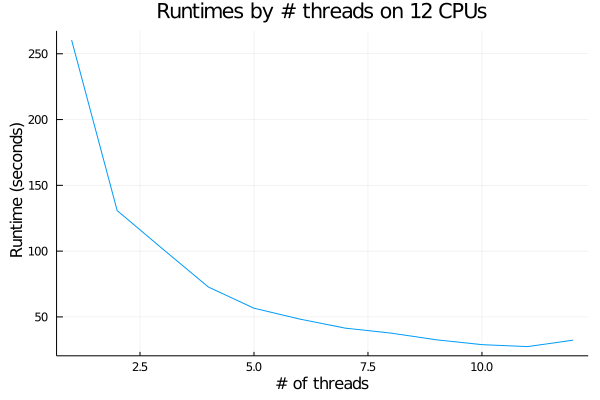
\includegraphics[scale=.35]{hw4_threads.png}
\end{figure}

\end{document}
